% Options for packages loaded elsewhere
\PassOptionsToPackage{unicode}{hyperref}
\PassOptionsToPackage{hyphens}{url}
\PassOptionsToPackage{dvipsnames,svgnames,x11names}{xcolor}
%
\documentclass[
  letterpaper,
  DIV=11,
  numbers=noendperiod]{scrartcl}

\usepackage{amsmath,amssymb}
\usepackage{iftex}
\ifPDFTeX
  \usepackage[T1]{fontenc}
  \usepackage[utf8]{inputenc}
  \usepackage{textcomp} % provide euro and other symbols
\else % if luatex or xetex
  \usepackage{unicode-math}
  \defaultfontfeatures{Scale=MatchLowercase}
  \defaultfontfeatures[\rmfamily]{Ligatures=TeX,Scale=1}
\fi
\usepackage{lmodern}
\ifPDFTeX\else  
    % xetex/luatex font selection
\fi
% Use upquote if available, for straight quotes in verbatim environments
\IfFileExists{upquote.sty}{\usepackage{upquote}}{}
\IfFileExists{microtype.sty}{% use microtype if available
  \usepackage[]{microtype}
  \UseMicrotypeSet[protrusion]{basicmath} % disable protrusion for tt fonts
}{}
\makeatletter
\@ifundefined{KOMAClassName}{% if non-KOMA class
  \IfFileExists{parskip.sty}{%
    \usepackage{parskip}
  }{% else
    \setlength{\parindent}{0pt}
    \setlength{\parskip}{6pt plus 2pt minus 1pt}}
}{% if KOMA class
  \KOMAoptions{parskip=half}}
\makeatother
\usepackage{xcolor}
\setlength{\emergencystretch}{3em} % prevent overfull lines
\setcounter{secnumdepth}{5}
% Make \paragraph and \subparagraph free-standing
\makeatletter
\ifx\paragraph\undefined\else
  \let\oldparagraph\paragraph
  \renewcommand{\paragraph}{
    \@ifstar
      \xxxParagraphStar
      \xxxParagraphNoStar
  }
  \newcommand{\xxxParagraphStar}[1]{\oldparagraph*{#1}\mbox{}}
  \newcommand{\xxxParagraphNoStar}[1]{\oldparagraph{#1}\mbox{}}
\fi
\ifx\subparagraph\undefined\else
  \let\oldsubparagraph\subparagraph
  \renewcommand{\subparagraph}{
    \@ifstar
      \xxxSubParagraphStar
      \xxxSubParagraphNoStar
  }
  \newcommand{\xxxSubParagraphStar}[1]{\oldsubparagraph*{#1}\mbox{}}
  \newcommand{\xxxSubParagraphNoStar}[1]{\oldsubparagraph{#1}\mbox{}}
\fi
\makeatother

\usepackage{color}
\usepackage{fancyvrb}
\newcommand{\VerbBar}{|}
\newcommand{\VERB}{\Verb[commandchars=\\\{\}]}
\DefineVerbatimEnvironment{Highlighting}{Verbatim}{commandchars=\\\{\}}
% Add ',fontsize=\small' for more characters per line
\usepackage{framed}
\definecolor{shadecolor}{RGB}{241,243,245}
\newenvironment{Shaded}{\begin{snugshade}}{\end{snugshade}}
\newcommand{\AlertTok}[1]{\textcolor[rgb]{0.68,0.00,0.00}{#1}}
\newcommand{\AnnotationTok}[1]{\textcolor[rgb]{0.37,0.37,0.37}{#1}}
\newcommand{\AttributeTok}[1]{\textcolor[rgb]{0.40,0.45,0.13}{#1}}
\newcommand{\BaseNTok}[1]{\textcolor[rgb]{0.68,0.00,0.00}{#1}}
\newcommand{\BuiltInTok}[1]{\textcolor[rgb]{0.00,0.23,0.31}{#1}}
\newcommand{\CharTok}[1]{\textcolor[rgb]{0.13,0.47,0.30}{#1}}
\newcommand{\CommentTok}[1]{\textcolor[rgb]{0.37,0.37,0.37}{#1}}
\newcommand{\CommentVarTok}[1]{\textcolor[rgb]{0.37,0.37,0.37}{\textit{#1}}}
\newcommand{\ConstantTok}[1]{\textcolor[rgb]{0.56,0.35,0.01}{#1}}
\newcommand{\ControlFlowTok}[1]{\textcolor[rgb]{0.00,0.23,0.31}{\textbf{#1}}}
\newcommand{\DataTypeTok}[1]{\textcolor[rgb]{0.68,0.00,0.00}{#1}}
\newcommand{\DecValTok}[1]{\textcolor[rgb]{0.68,0.00,0.00}{#1}}
\newcommand{\DocumentationTok}[1]{\textcolor[rgb]{0.37,0.37,0.37}{\textit{#1}}}
\newcommand{\ErrorTok}[1]{\textcolor[rgb]{0.68,0.00,0.00}{#1}}
\newcommand{\ExtensionTok}[1]{\textcolor[rgb]{0.00,0.23,0.31}{#1}}
\newcommand{\FloatTok}[1]{\textcolor[rgb]{0.68,0.00,0.00}{#1}}
\newcommand{\FunctionTok}[1]{\textcolor[rgb]{0.28,0.35,0.67}{#1}}
\newcommand{\ImportTok}[1]{\textcolor[rgb]{0.00,0.46,0.62}{#1}}
\newcommand{\InformationTok}[1]{\textcolor[rgb]{0.37,0.37,0.37}{#1}}
\newcommand{\KeywordTok}[1]{\textcolor[rgb]{0.00,0.23,0.31}{\textbf{#1}}}
\newcommand{\NormalTok}[1]{\textcolor[rgb]{0.00,0.23,0.31}{#1}}
\newcommand{\OperatorTok}[1]{\textcolor[rgb]{0.37,0.37,0.37}{#1}}
\newcommand{\OtherTok}[1]{\textcolor[rgb]{0.00,0.23,0.31}{#1}}
\newcommand{\PreprocessorTok}[1]{\textcolor[rgb]{0.68,0.00,0.00}{#1}}
\newcommand{\RegionMarkerTok}[1]{\textcolor[rgb]{0.00,0.23,0.31}{#1}}
\newcommand{\SpecialCharTok}[1]{\textcolor[rgb]{0.37,0.37,0.37}{#1}}
\newcommand{\SpecialStringTok}[1]{\textcolor[rgb]{0.13,0.47,0.30}{#1}}
\newcommand{\StringTok}[1]{\textcolor[rgb]{0.13,0.47,0.30}{#1}}
\newcommand{\VariableTok}[1]{\textcolor[rgb]{0.07,0.07,0.07}{#1}}
\newcommand{\VerbatimStringTok}[1]{\textcolor[rgb]{0.13,0.47,0.30}{#1}}
\newcommand{\WarningTok}[1]{\textcolor[rgb]{0.37,0.37,0.37}{\textit{#1}}}

\providecommand{\tightlist}{%
  \setlength{\itemsep}{0pt}\setlength{\parskip}{0pt}}\usepackage{longtable,booktabs,array}
\usepackage{calc} % for calculating minipage widths
% Correct order of tables after \paragraph or \subparagraph
\usepackage{etoolbox}
\makeatletter
\patchcmd\longtable{\par}{\if@noskipsec\mbox{}\fi\par}{}{}
\makeatother
% Allow footnotes in longtable head/foot
\IfFileExists{footnotehyper.sty}{\usepackage{footnotehyper}}{\usepackage{footnote}}
\makesavenoteenv{longtable}
\usepackage{graphicx}
\makeatletter
\def\maxwidth{\ifdim\Gin@nat@width>\linewidth\linewidth\else\Gin@nat@width\fi}
\def\maxheight{\ifdim\Gin@nat@height>\textheight\textheight\else\Gin@nat@height\fi}
\makeatother
% Scale images if necessary, so that they will not overflow the page
% margins by default, and it is still possible to overwrite the defaults
% using explicit options in \includegraphics[width, height, ...]{}
\setkeys{Gin}{width=\maxwidth,height=\maxheight,keepaspectratio}
% Set default figure placement to htbp
\makeatletter
\def\fps@figure{htbp}
\makeatother

\KOMAoption{captions}{tableheading}
\makeatletter
\@ifpackageloaded{caption}{}{\usepackage{caption}}
\AtBeginDocument{%
\ifdefined\contentsname
  \renewcommand*\contentsname{Table of contents}
\else
  \newcommand\contentsname{Table of contents}
\fi
\ifdefined\listfigurename
  \renewcommand*\listfigurename{List of Figures}
\else
  \newcommand\listfigurename{List of Figures}
\fi
\ifdefined\listtablename
  \renewcommand*\listtablename{List of Tables}
\else
  \newcommand\listtablename{List of Tables}
\fi
\ifdefined\figurename
  \renewcommand*\figurename{Figure}
\else
  \newcommand\figurename{Figure}
\fi
\ifdefined\tablename
  \renewcommand*\tablename{Table}
\else
  \newcommand\tablename{Table}
\fi
}
\@ifpackageloaded{float}{}{\usepackage{float}}
\floatstyle{ruled}
\@ifundefined{c@chapter}{\newfloat{codelisting}{h}{lop}}{\newfloat{codelisting}{h}{lop}[chapter]}
\floatname{codelisting}{Listing}
\newcommand*\listoflistings{\listof{codelisting}{List of Listings}}
\makeatother
\makeatletter
\makeatother
\makeatletter
\@ifpackageloaded{caption}{}{\usepackage{caption}}
\@ifpackageloaded{subcaption}{}{\usepackage{subcaption}}
\makeatother

\ifLuaTeX
  \usepackage{selnolig}  % disable illegal ligatures
\fi
\usepackage{bookmark}

\IfFileExists{xurl.sty}{\usepackage{xurl}}{} % add URL line breaks if available
\urlstyle{same} % disable monospaced font for URLs
\hypersetup{
  pdftitle={Mckinney Fire Metabolism: Depth Model},
  pdfauthor={Laurel Genzoli},
  colorlinks=true,
  linkcolor={blue},
  filecolor={Maroon},
  citecolor={Blue},
  urlcolor={Blue},
  pdfcreator={LaTeX via pandoc}}


\title{Mckinney Fire Metabolism: Depth Model}
\author{Laurel Genzoli}
\date{2025-07-31}

\begin{document}
\maketitle

\renewcommand*\contentsname{Table of contents}
{
\hypersetup{linkcolor=}
\setcounter{tocdepth}{3}
\tableofcontents
}

\section{Script Descriptioins}\label{script-descriptioins}

This script creates a depth model for the Seiad Valley reach of the
Klamath River. Using data from the Bradley Model and the Yurok Tribe
Topo LiDAR data, we obtain depth measurements from throughout the river
by calculating the difference between bed and water elevation across the
full range of flows explored in Bradly model. We fit a power
relationship between depth and flow and then used this model to estimate
mean reach depth daily based on mean daily discharge in the metabolism
data set. Scaling metabolism to depth was done as a final step in them
``metab\_QA'' script.

\subsection{Packages \& Data}\label{packages-data}

\begin{Shaded}
\begin{Highlighting}[]
\FunctionTok{setwd}\NormalTok{(}\StringTok{\textquotesingle{}/Users/laurelgenzoli/Dropbox/2024\_Projects/Mckinney\_Fire\_Metab/Mck{-}Fire{-}Metab{-}GH\textquotesingle{}}\NormalTok{)}

\FunctionTok{library}\NormalTok{(brms)}
\FunctionTok{library}\NormalTok{(loo)}
\FunctionTok{library}\NormalTok{(tidybayes)}
\FunctionTok{library}\NormalTok{(tidyverse)}
\FunctionTok{library}\NormalTok{(ggplot2)}
\FunctionTok{library}\NormalTok{(fs)}
\FunctionTok{library}\NormalTok{(cowplot)}
\end{Highlighting}
\end{Shaded}

\subsubsection{Load dense mesh data (lower
flows)}\label{load-dense-mesh-data-lower-flows}

The Bradley model used a dense mesh at the lower flows for modeling bed
and water surface elevations.

\begin{verbatim}
         z
1 7.690163
\end{verbatim}

\subsubsection{Read in coarse mesh (higher
flows)}\label{read-in-coarse-mesh-higher-flows}

Only coarse mesh data was available for the higher flow (flood) data

\subsection{Full data frame of depth
estimates}\label{full-data-frame-of-depth-estimates}

We use depth ranging from a 75\% exceedance probability to a 10 year
flood interval. Our metabolism data set spans discharge from 945 to
17,600 cfs, the higher end of which corresponds to a 2-year flood
interval.

The flows for each exceedance probability/flood return interval are from
Bradley 2021: ``Bradley, N. D. 2021. Klamath River hydraulic model: Iron
Gate Dam to the Pacific Ocean. U.S. Department of the Interior,
Technical Report No.~ENV-2021-066. U.S. Bureau of Reclamation''

For the fine mesh we had \textgreater1900 estimates of depth and for
coarse mesh, \textgreater800 within our 10-km reach length extending
from the Seiad Sonde to 10-km upriver.

Here, we average depths across the reach of each exceedance flow in the
model, convert from standard units to metric, and also extract the depth
extending 10 and 20 km upriver to be used as a quick sensitivey analysis
for our choice of reach length (below).

\begin{verbatim}
# A tibble: 7 x 4
  ex.prob    reach.z ex.flow.cfs ex.flow.cms
  <fct>        <dbl>       <dbl>       <dbl>
1 75_Percent    1.21        1320        37.4
2 50_Percent    1.37        1870        53.0
3 25_Percent    1.74        3400        96.3
4 10_Percent    2.34        6800       193. 
5 2_YrFlood     3.80       17600       498. 
6 5_YrFlood     5.65       39960      1132. 
7 10_YrFlood    6.78       56540      1601. 
\end{verbatim}

\subsubsection{Depth distributions and depth-flow
relationship}\label{depth-distributions-and-depth-flow-relationship}

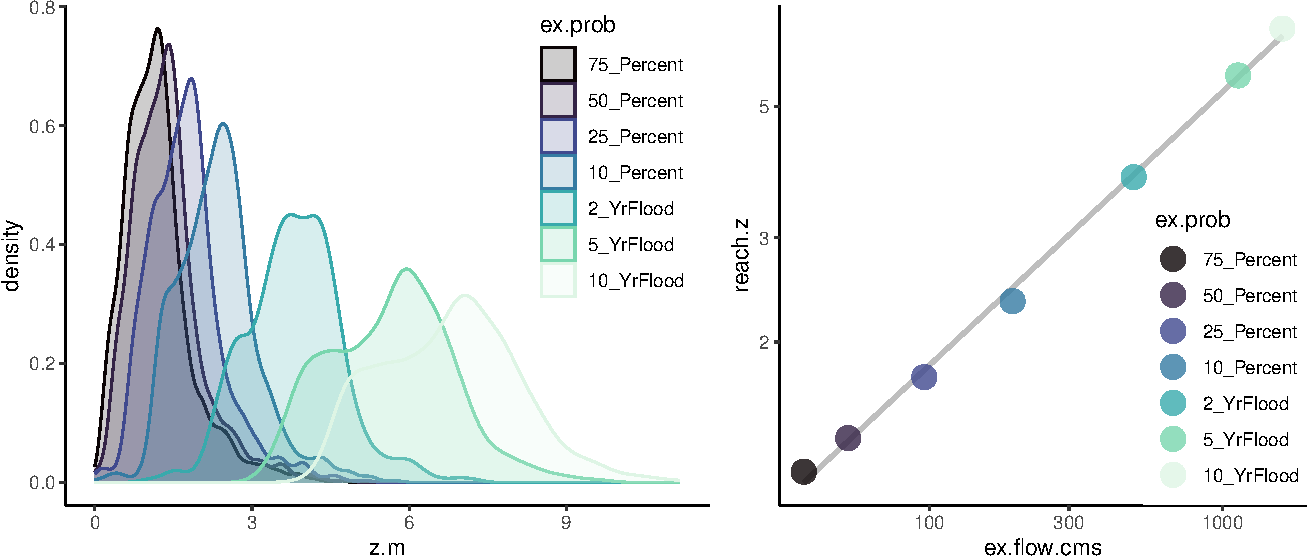
\includegraphics{Depth_model_files/figure-pdf/unnamed-chunk-5-1.pdf}

\subsection{Sensitvity analysis of reach
length}\label{sensitvity-analysis-of-reach-length}

The choice of 10 vs.~20 km changes reach depths very little. There is
some deviation of mean reach depth between the 10 and 20 km reach at
flood flows, but our data set tops out at the flows of a 2-year flood,
so we are using a 10 km reach length to estimates reach depths.

\begin{center}
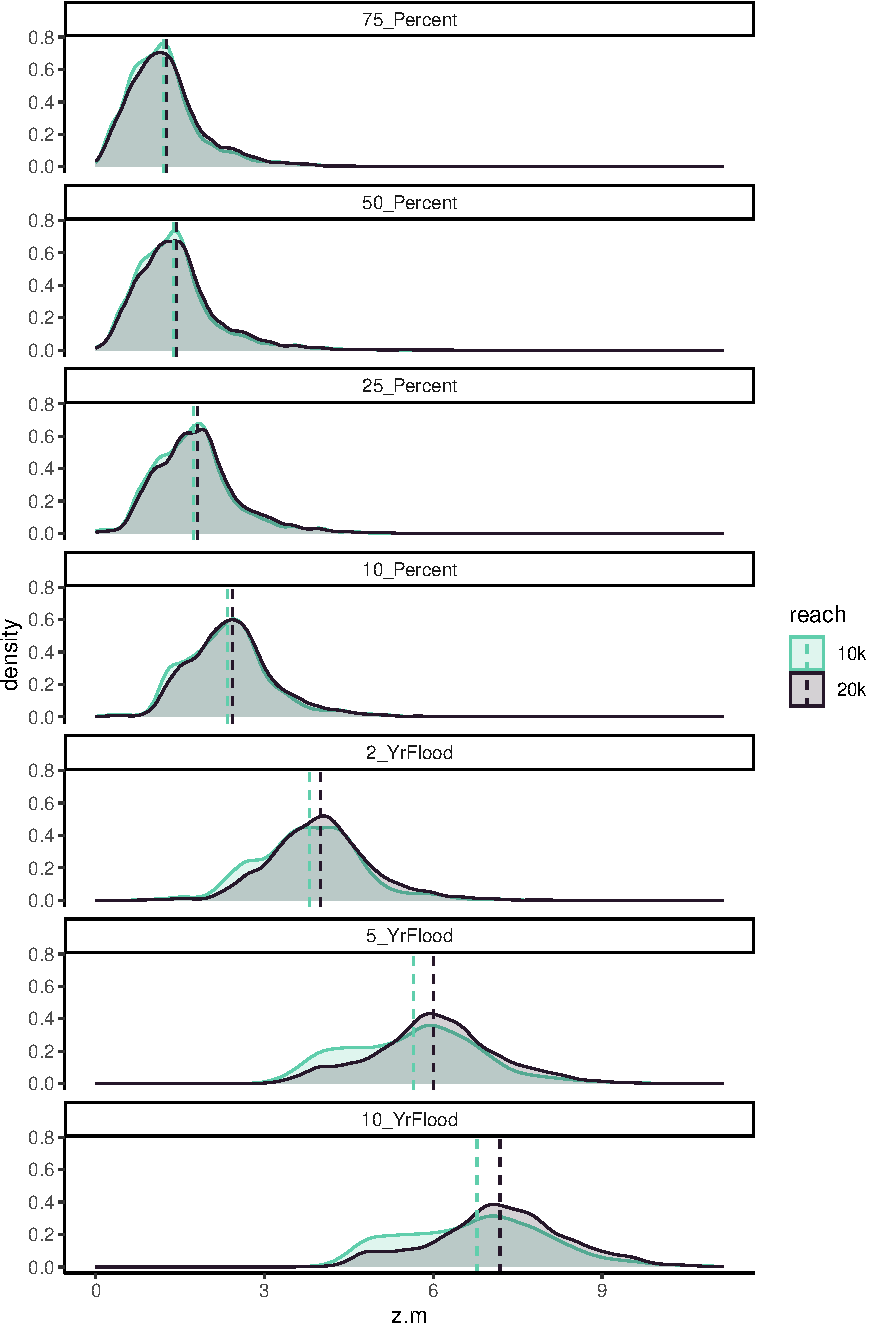
\includegraphics{Depth_model_files/figure-pdf/unnamed-chunk-6-1.pdf}
\end{center}

\subsection{Final model for depth
estimation}\label{final-model-for-depth-estimation}

This model will be used to estimate a daily mean reach depth, which is
used to scale metabolism to aerial units daily with changing flow
conditions. Metabolism is adjusted to depth in the ``metab\_QA'' script.

\(log(z) = -1.47 + log(Q) \times 0.45\)

\begin{verbatim}

Call:
lm(formula = log(reach.z) ~ log(ex.flow.cms), data = depth.sum)

Residuals:
        1         2         3         4         5         6         7 
 0.041954  0.011544 -0.027494 -0.052424 -0.009528  0.007076  0.028871 

Coefficients:
                  Estimate Std. Error t value Pr(>|t|)    
(Intercept)      -1.531144   0.055172  -27.75 1.14e-06 ***
log(ex.flow.cms)  0.462973   0.009845   47.03 8.21e-08 ***
---
Signif. codes:  0 '***' 0.001 '**' 0.01 '*' 0.05 '.' 0.1 ' ' 1

Residual standard error: 0.0357 on 5 degrees of freedom
Multiple R-squared:  0.9977,    Adjusted R-squared:  0.9973 
F-statistic:  2212 on 1 and 5 DF,  p-value: 8.211e-08
\end{verbatim}




\end{document}
